\hypertarget{product_8inc}{
\section{include/product.inc File Reference}
\label{product_8inc}\index{include/product.inc@{include/product.inc}}
}
Functions to output Product Info. 

\subsection*{Functions}
\begin{CompactItemize}
\item 
\hyperlink{product_8inc_ac7b378120072ec50fd998c962a419a2}{getImages} (\$product, \$type= 'generic')
\end{CompactItemize}


\subsection{Detailed Description}
Functions to output Product Info. 

Various pieces of info gleamed from the web will be handled by functions contained in this file. Currently, it only handles getting product images 

Definition in file \hyperlink{product_8inc-source}{product.inc}.

\subsection{Function Documentation}
\hypertarget{product_8inc_ac7b378120072ec50fd998c962a419a2}{
\index{product.inc@{product.inc}!getImages@{getImages}}
\index{getImages@{getImages}!product.inc@{product.inc}}
\subsubsection{\setlength{\rightskip}{0pt plus 5cm}getImages (\$ {\em product}, \$ {\em type} = {\tt 'generic'})}}
\label{product_8inc_ac7b378120072ec50fd998c962a419a2}


Gets Appropriate Images from google Image Search \begin{Desc}
\item[Parameters:]
\begin{description}
\item[{\em \$product}]The product to get images for \item[{\em \$type}]The Product type to search for, defaults to a generic product. If it is a book, \char`\"{}book\char`\"{} is appended to the search query to narrow the result to what should be book covers. \end{description}
\end{Desc}
\begin{Desc}
\item[Returns:]HTML code to output product images \end{Desc}


Definition at line 18 of file product.inc.

References fget().

Referenced by getBarcodeInfo().

\begin{Code}\begin{verbatim}18                                                 {
22   $q = '';
23   switch ($type) {
24     case 'generic':
25       $q = urlencode("\"$product\"");
26       break;
27     case 'book':
28       $q = urlencode("\"$product\" book");
29       break;
30   }
34   $json = json_decode(fget('http://ajax.googleapis.com/ajax/services/search/images?v=1.0&q=' . $q . '&rsz=large'));
35 
36   // Hack to get Indexes working
37   if ($_GET['index']) {
38     $currentIndex = (int) $_GET['index'];
39   }
40   else {
41     $currentIndex = 0;
42   }
43   $prevIndex = $currentIndex - 1;
44   $nextIndex = $currentIndex + 1;
45   $i = 0;
46   $getText = '?';
47   foreach ($_GET as $item) {
48     if (key($_GET) != 'index') {
49       if ($i == 0) {
50         $getText .= key($_GET) . '=' . $item;
51       }
52       else {
53         $getText .= '&' . key($_GET) . '=' . $item;
54       }
55     }
56     next($_GET);
57     $i++;
58   }
59 
60   $originalContextUrl = $json->responseData->results[$currentIndex]->originalContextUrl;
61   $imgSrc = $json->responseData->results[$currentIndex]->tbUrl;
62   $visibleUrl = $json->responseData->results[$currentIndex]->visibleUrl;
63 
67   $output = "<div id=\"prodimg\">";
68   // Only display previous button if there are previous values
69   if ($currentIndex > 0) {
70     $output .= "<a href=\"{$getText}&index={$prevIndex}\"><img src=\"images/arrows/left.png\" alt=\"Previous Image\" title=\"Previous Image\" /></a>";
71   }
72   $output .= "<a href=\"{$originalContextUrl}\" target=\"_blank\"><img src=\"{$imgSrc}\" alt=\"Image of $product From {$visibleUrl}\" title=\"Image of $product From {$visibleUrl}\" id=\"prodimg\"></a>";
73   // Only display next button if there are more images
74   if ($currentIndex < count($json->responseData->results) - 1) {
75    $output .= "<a href=\"{$getText}&index={$nextIndex}\"> <img src=\"images/arrows/right.png\" alt=\"Next Image\" title=\"Next Image\" /></a><br /><a href=\"aboutimages.html\" target=\"_blank\" onclick=\"popup(this.href, 200, 300); return false;\">About this image</a></div>";
76   }
77 
78   return $output;
79 }
\end{verbatim}
\end{Code}




Here is the call graph for this function:\nopagebreak
\begin{figure}[H]
\begin{center}
\leavevmode
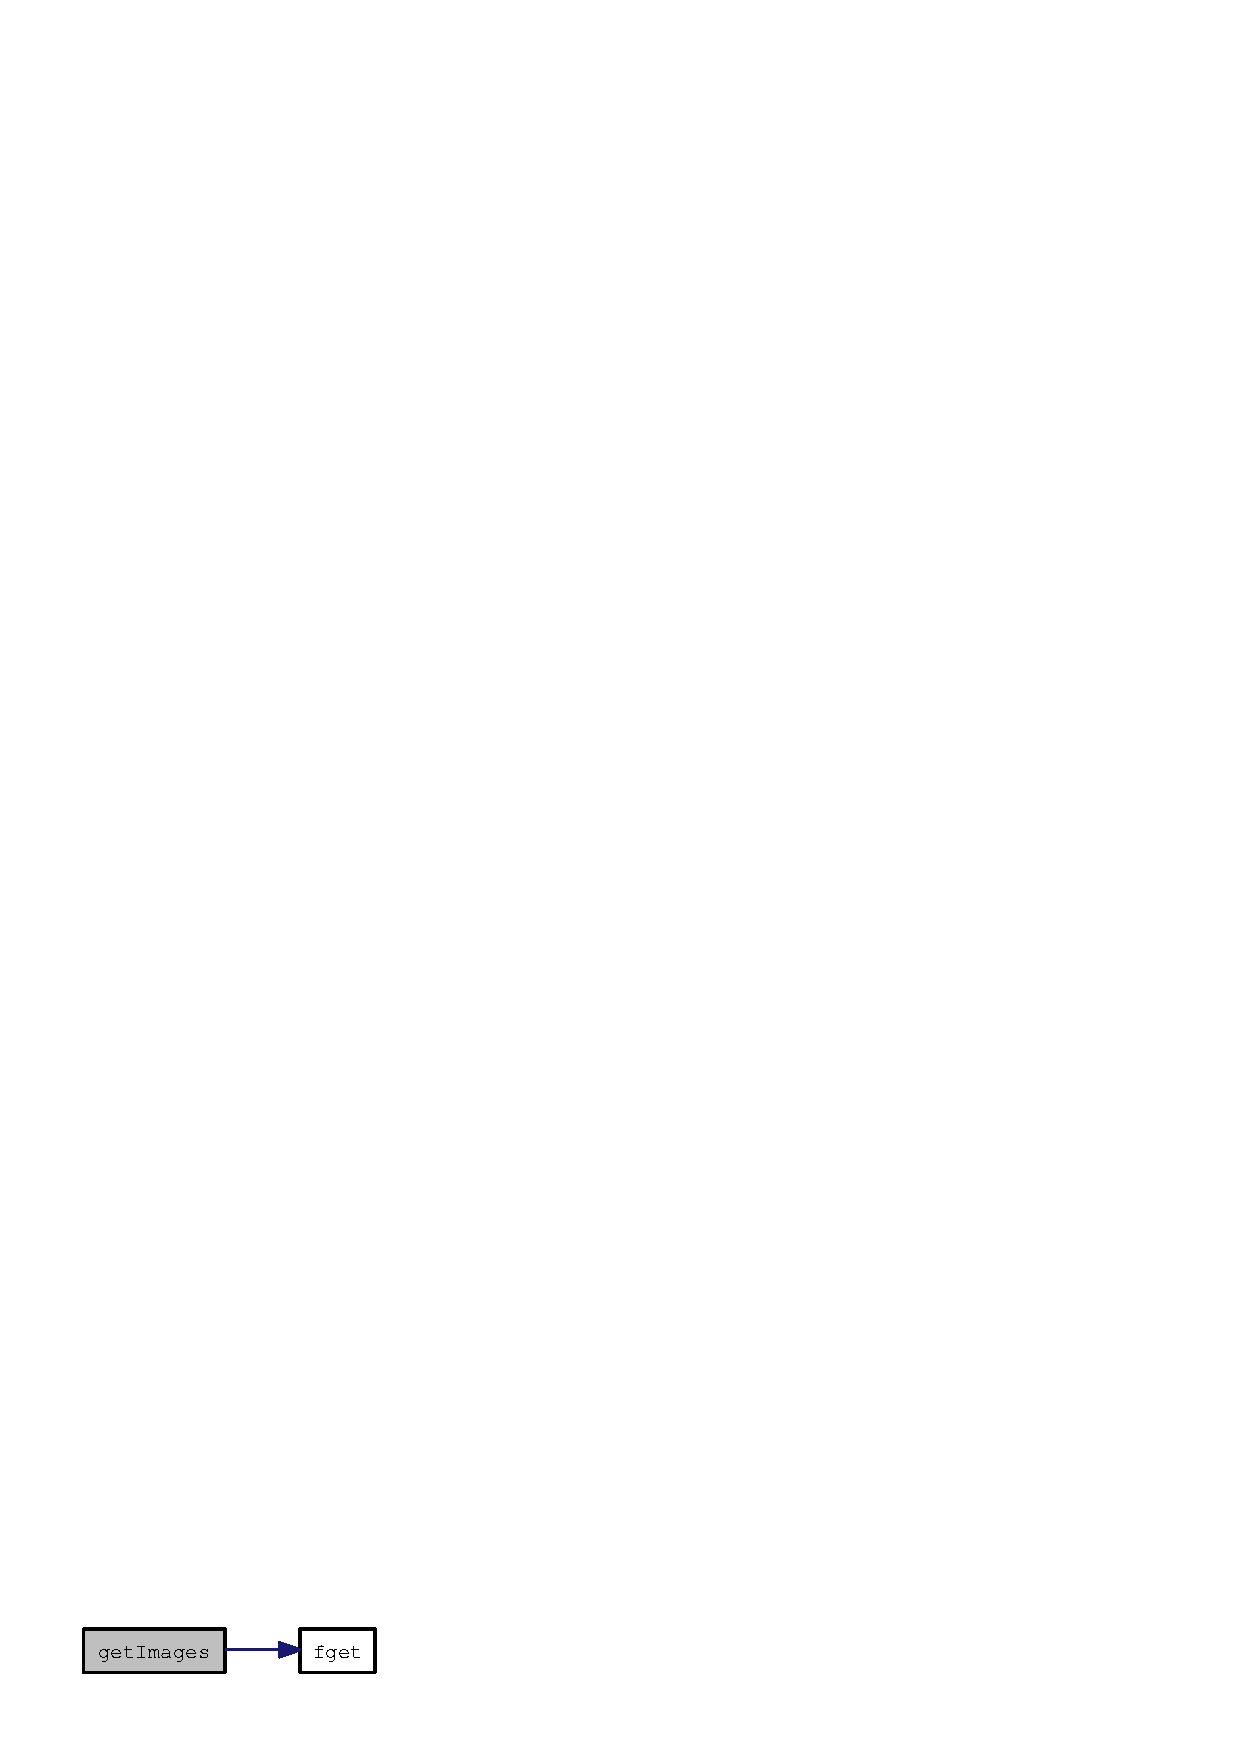
\includegraphics[width=92pt]{product_8inc_ac7b378120072ec50fd998c962a419a2_cgraph}
\end{center}
\end{figure}


Here is the caller graph for this function:\nopagebreak
\begin{figure}[H]
\begin{center}
\leavevmode
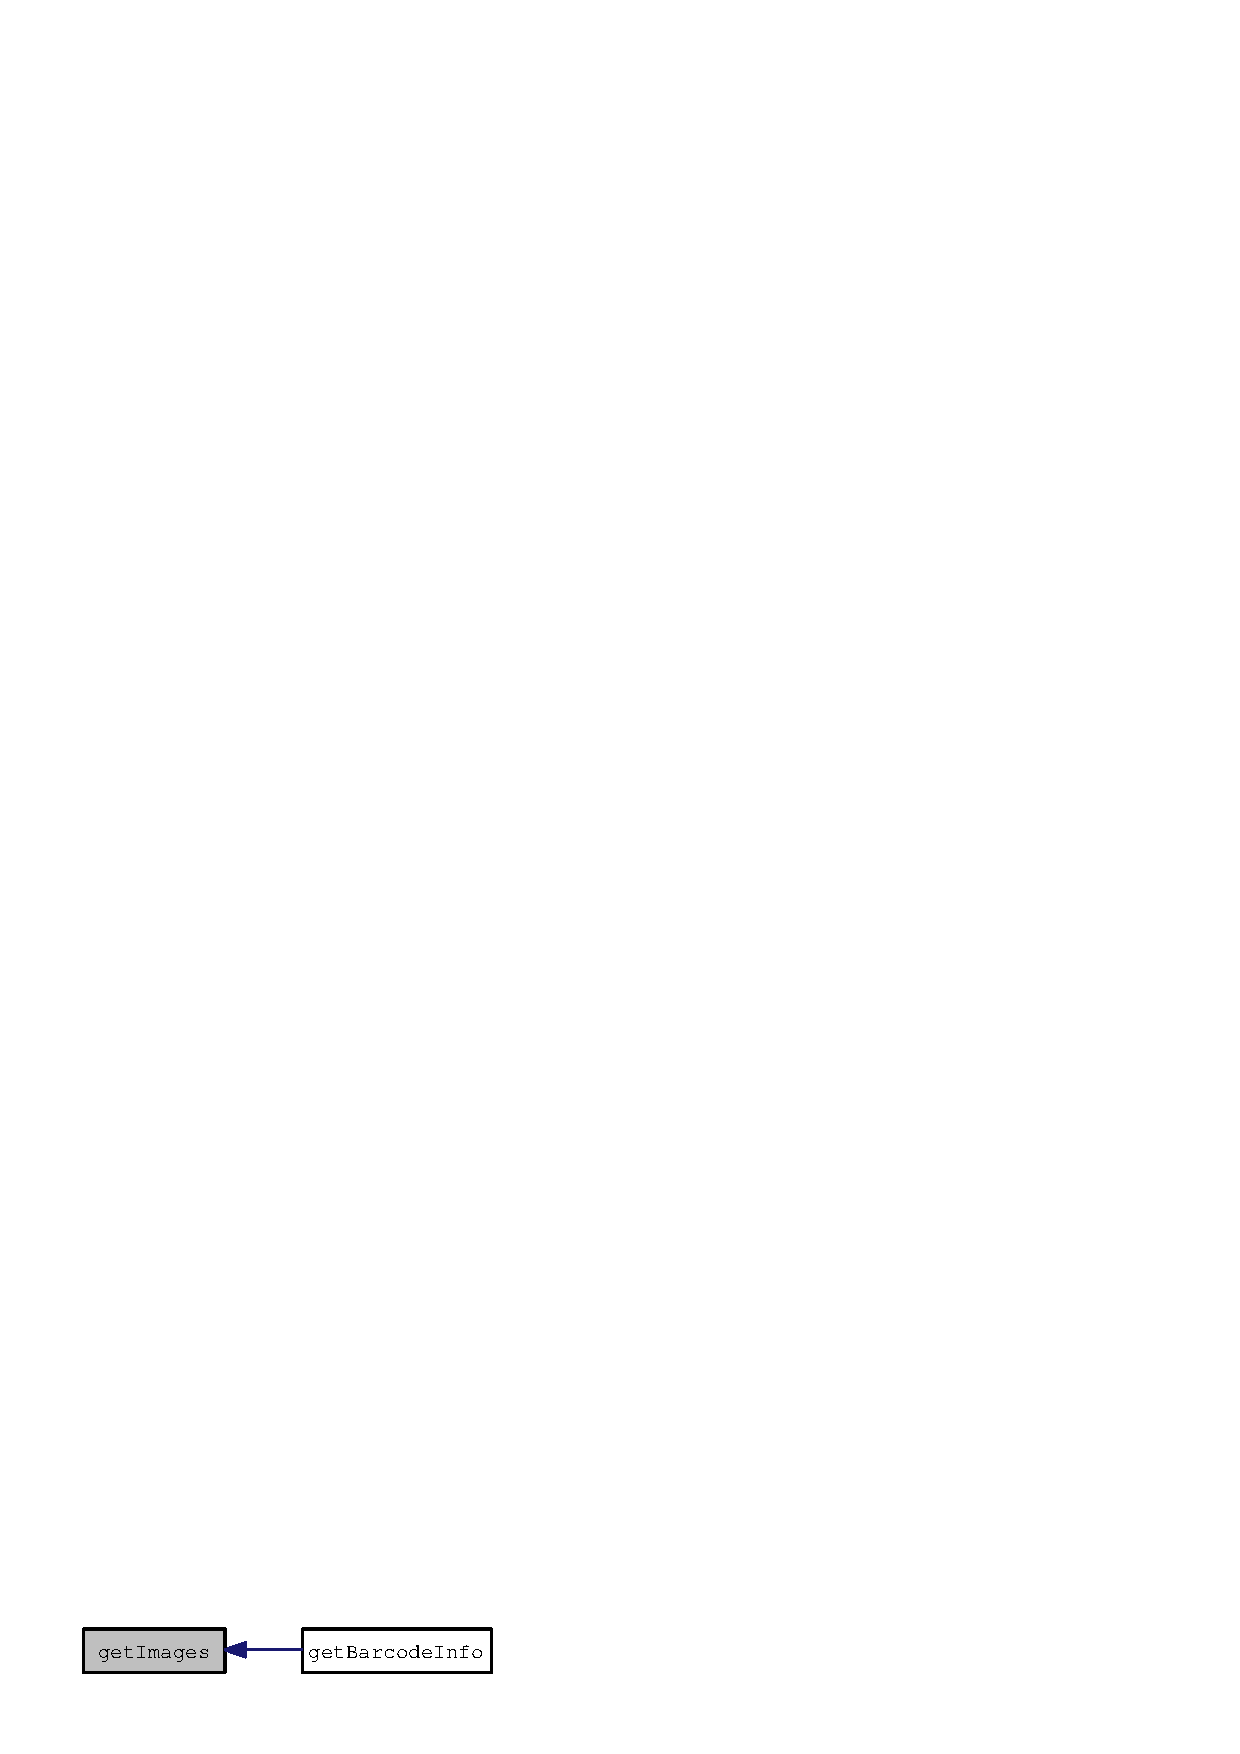
\includegraphics[width=120pt]{product_8inc_ac7b378120072ec50fd998c962a419a2_icgraph}
\end{center}
\end{figure}
